\chapter{Huffmantræ} \label{chapter:appendiks}
Følgende figurer beskriver trinnene i skabelsen af Huffmantræet i afsnit \vref{sec:huffmanteori}.
\begin{figure}[!h]
\centering
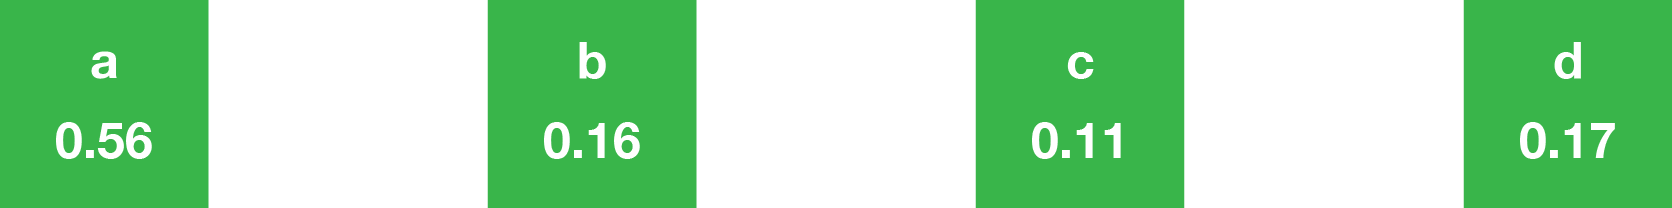
\includegraphics[width=0.5\textwidth]{Billeder/Huffman-tree-ex-01.png}
\caption{Første trin i skabelsen af Huffmantræ}
\label{fig:huffmantrae_ex1}
\end{figure}
\hfill
\begin{figure}[!h]
\centering
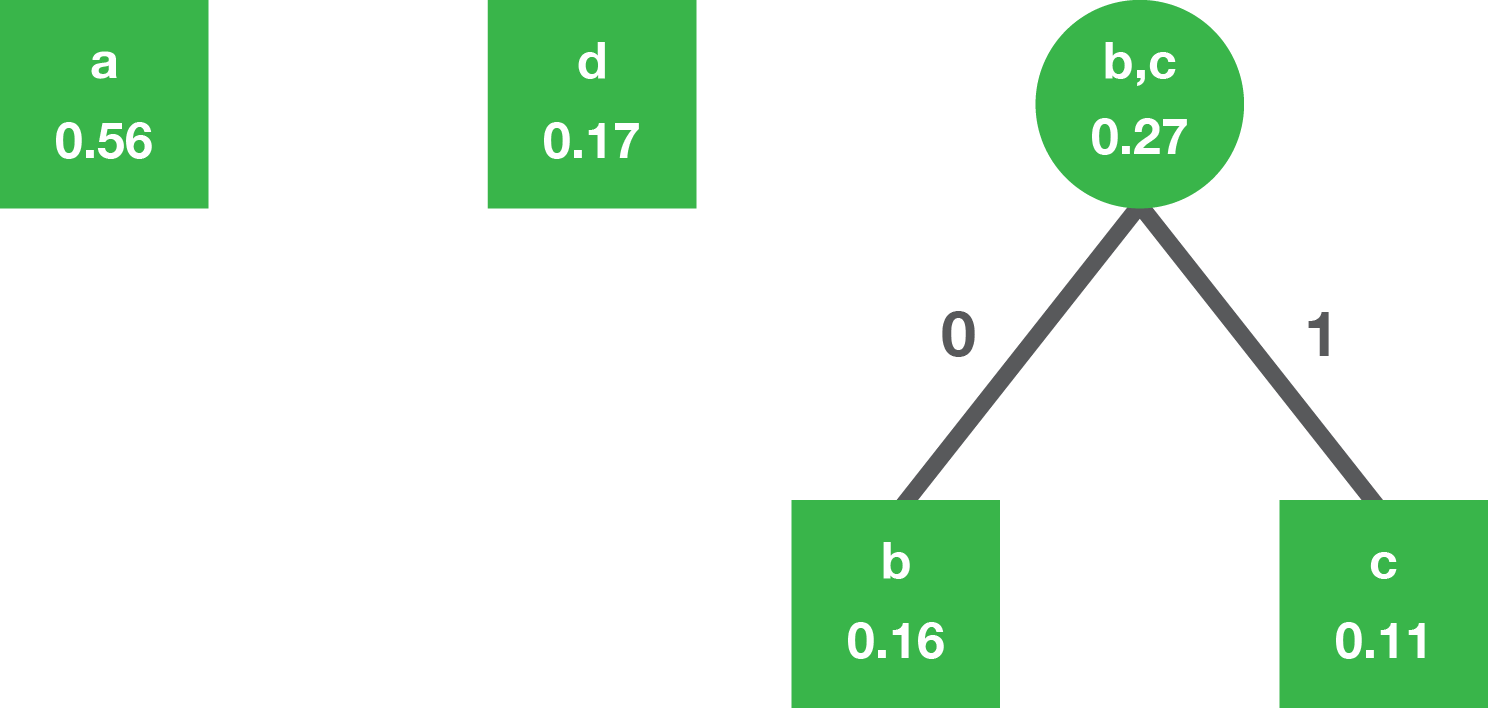
\includegraphics[width=0.5\textwidth]{Billeder/Huffman-tree-ex-02.png}
\caption{Andet trin i skabelsen af Huffmantræ}
\label{fig:huffmantrae_ex2}
\end{figure}
\begin{figure}[!h]
\begin{minipage}{0.45\textwidth}
\centering
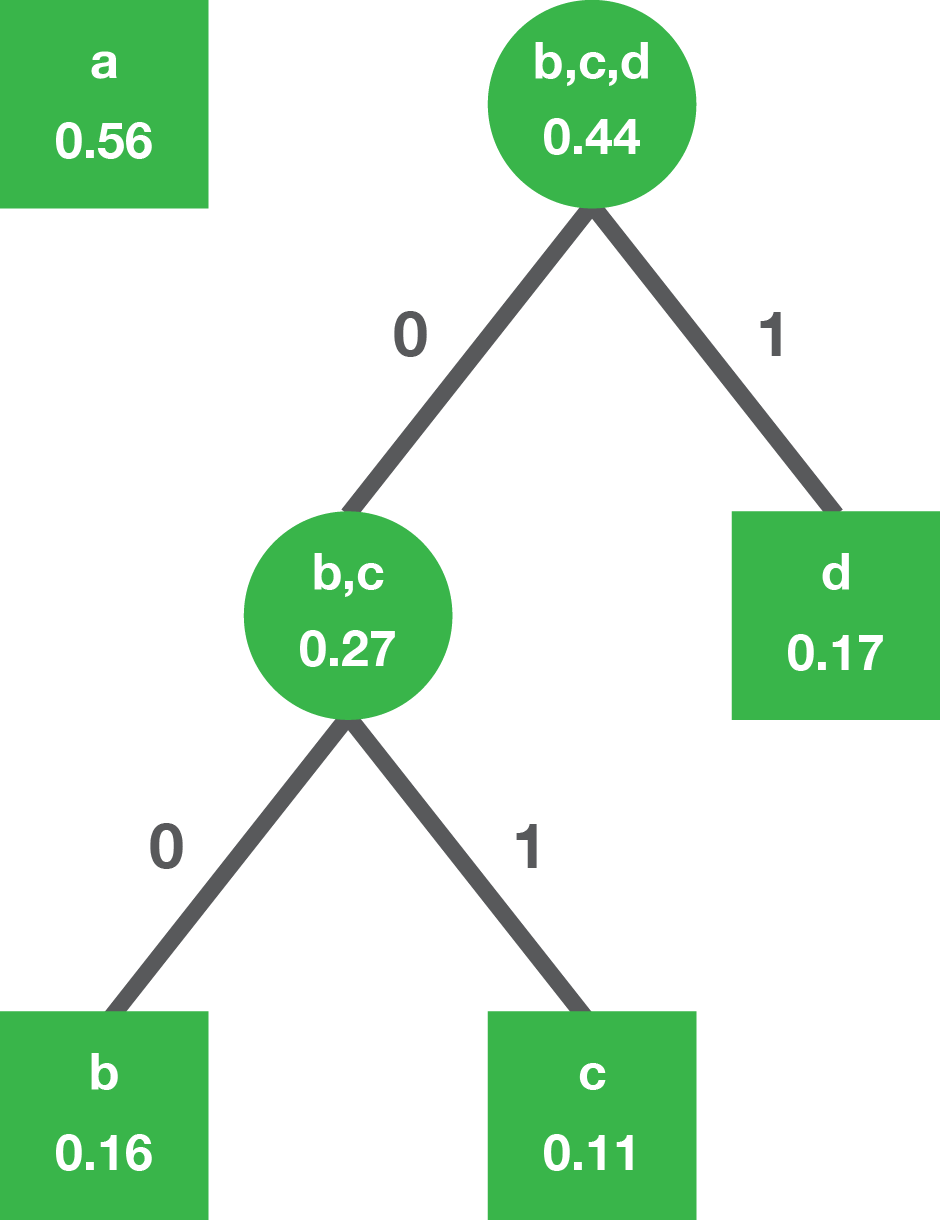
\includegraphics[width=0.6\linewidth]{Billeder/Huffman-tree-ex-03.png}
\caption{Tredje trin i skabelsen af Huffmantræ}
\label{fig:huffmantrae_ex3}
\end{minipage}
\hspace{0.5cm}
\begin{minipage}{0.45\textwidth}
\centering
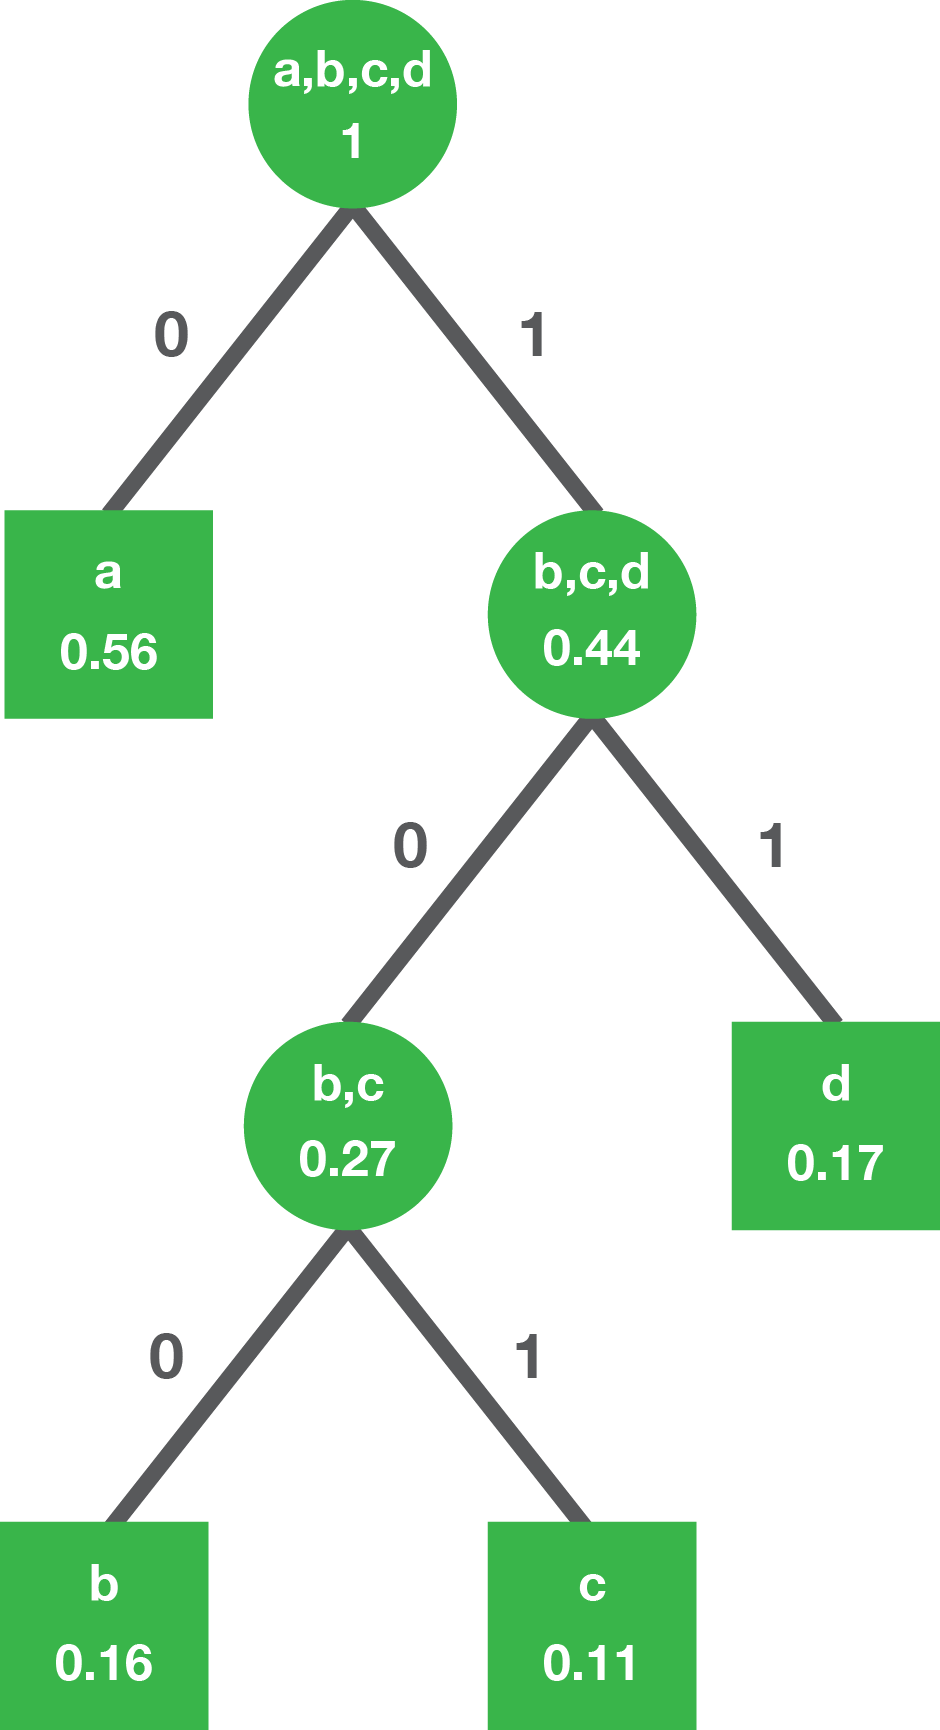
\includegraphics[width=0.6\linewidth]{Billeder/Huffman-tree-ex-04.png}
\caption{Fjerde trin i skabelsen af Huffmantræ}
\label{fig:huffmantrae_ex4}
\end{minipage}
\end{figure}